\section{Hiện thực hệ thống}
\subsection{Kiến trúc hiện thực hệ thống}
Mục này trình bày kiến trúc hiện thực của hệ thống FoodTour Planner, mô tả cách các
thành phần phần mềm được tổ chức và tương tác với nhau trong quá trình vận hành.
Dựa trên kết quả phân tích và thiết kế ở chương trước, hệ thống được triển khai theo
mô hình kiến trúc nhiều tầng , tách biệt rõ ràng giữa giao diện người dùng, tầng xử lý nghiệp vụ và tầng dữ liệu nhằm đảm bảo tính mở rộng, dễ bảo trì và linh hoạt trong phát triển.
\subsubsection{Phân tích kiến trúc tổng thể}
Hình 6.1 minh họa kiến trúc tổng thể của hệ thống. Về mặt logic, hệ thống được chia
thành bốn thành phần chính: Browser, Web Frontend, Backend Service và Database.
\begin{figure}[H]
    \centering
    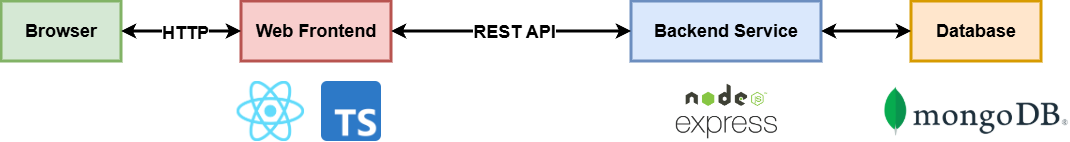
\includegraphics[width=0.85\linewidth]{img/6.png}
    \caption{System Architecture}
\end{figure}
Người dùng truy cập hệ thống thông qua trình duyệt (Browser), nơi các yêu cầu được
gửi đến Web Frontend thông qua giao thức HTTP. Web Frontend đóng vai trò hiển thị
giao diện và xử lý tương tác người dùng, đồng thời gửi các yêu cầu nghiệp vụ đến
Backend Service thông qua các API theo chuẩn REST.

Backend Service chịu trách nhiệm xử lý logic nghiệp vụ của hệ thống như xác thực
người dùng, tìm kiếm quán ăn, quản lý food tour, xử lý đánh giá và phân quyền quản trị.
Các thao tác đọc/ghi dữ liệu được thực hiện thông qua việc giao tiếp với hệ quản trị
cơ sở dữ liệu. Tầng Database đảm nhiệm việc lưu trữ và truy xuất dữ liệu lâu dài của
hệ thống.

\subsubsection{Công nghệ sử dụng trong hệ thống}
\subsubsubsection{React và TypeScript – Tầng giao diện người dùng}
React là một thư viện JavaScript được Facebook giới thiệu vào năm 2013, hỗ trợ xây dựng giao diện người dùng dựa trên các thành phần (component-based). React cho phép tái sử dụng giao diện, cập nhật trạng thái hiệu quả và phù hợp với mô hình Single Page Application (SPA).

TypeScript, do Microsoft phát triển và ra mắt năm 2012, là một phần mở rộng của JavaScript với khả năng kiểm tra kiểu tĩnh. Việc sử dụng TypeScript giúp giảm lỗi trong quá trình phát triển, tăng khả năng đọc hiểu và bảo trì mã nguồn.

Việc lựa chọn React cho tầng giao diện giúp hệ thống dễ dàng xây dựng các màn hình
tương tác phức tạp như tìm kiếm quán ăn, quản lý food tour và hiển thị bản đồ lộ trình.
Mô hình component-based của React hỗ trợ tái sử dụng giao diện, giảm trùng lặp mã nguồn
và thuận tiện cho việc mở rộng chức năng.

Bên cạnh đó, TypeScript giúp phát hiện sớm các lỗi liên quan đến kiểu dữ liệu trong quá
trình phát triển, đặc biệt hữu ích khi hệ thống có nhiều module và luồng dữ liệu phức tạp.
Việc kết hợp React và TypeScript góp phần nâng cao chất lượng mã nguồn và khả năng
bảo trì của hệ thống.
\subsubsubsection{Node.js và Express – Tầng backend}

Node.js được giới thiệu vào năm 2009, là một nền tảng chạy JavaScript phía server dựa trên engine V8 của Google. Node.js hỗ trợ mô hình xử lý bất đồng bộ (non-blocking I/O), cho phép hệ thống xử lý nhiều yêu cầu đồng thời với hiệu quả cao, đặc biệt phù hợp với các ứng dụng web thời gian thực.

Express là một framework web nhẹ chạy trên Node.js, cung cấp các cơ chế định tuyến (routing), middleware và xử lý request/response theo chuẩn REST. Trong hệ thống FoodTour Planner, Node.js kết hợp với Express được sử dụng để xây dựng các REST API phục vụ cho các chức năng như xác thực người dùng, tìm kiếm quán ăn, quản lý food tour và xử lý đánh giá.

So với các mô hình backend truyền thống xử lý đồng bộ, Node.js với cơ chế bất đồng bộ
giúp hệ thống sử dụng tài nguyên hiệu quả hơn khi xử lý nhiều yêu cầu đồng thời, đặc biệt
phù hợp với các ứng dụng web có nhiều thao tác truy vấn dữ liệu và tương tác người dùng.
Express cung cấp cấu trúc gọn nhẹ, dễ tổ chức các API theo module, phù hợp với kiến trúc
phân tầng được đề xuất trong hệ thống.

Việc sử dụng Node.js và Express cũng tạo sự thống nhất về ngôn ngữ lập trình giữa frontend
và backend, giúp giảm chi phí học tập và tăng hiệu quả phát triển trong phạm vi luận văn.
\subsubsubsection{MongoDB – Hệ quản trị cơ sở dữ liệu}
MongoDB là một hệ quản trị cơ sở dữ liệu NoSQL hướng document, được giới thiệu lần đầu
vào năm 2009 bởi công ty MongoDB Inc. Khác với các hệ quản trị cơ sở dữ liệu quan hệ
truyền thống, MongoDB lưu trữ dữ liệu dưới dạng các document có cấu trúc JSON/BSON,
cho phép biểu diễn dữ liệu linh hoạt và dễ dàng mở rộng theo yêu cầu nghiệp vụ.

Một đặc điểm quan trọng của MongoDB là khả năng hỗ trợ schema linh hoạt, trong đó các
document trong cùng một collection không bắt buộc phải có cấu trúc hoàn toàn giống nhau.
Điều này đặc biệt phù hợp với các hệ thống web hiện đại, nơi yêu cầu nghiệp vụ và mô hình
dữ liệu có thể thay đổi theo thời gian. Bên cạnh đó, MongoDB hỗ trợ tốt việc lưu trữ dữ liệu
lồng nhau (nested documents) và các danh sách (arrays), giúp giảm sự phụ thuộc vào các
phép join phức tạp thường gặp trong mô hình cơ sở dữ liệu quan hệ.

Đối với hệ thống FoodTour Planner, dữ liệu mang tính bán cấu trúc và có mối quan hệ linh
hoạt, chẳng hạn như danh sách quán ăn trong một food tour, các điểm dừng theo thứ tự,
đánh giá kèm hình ảnh, hoặc thông tin khẩu vị cá nhân của người dùng. Việc sử dụng
MongoDB cho phép biểu diễn các cấu trúc này một cách tự nhiên dưới dạng document,
đồng thời giúp quá trình truy vấn, cập nhật và mở rộng dữ liệu trở nên thuận tiện hơn khi
bổ sung thêm chức năng hoặc thuộc tính mới.

Ngoài ra, MongoDB hỗ trợ hiệu quả các thao tác đọc dữ liệu theo dạng danh sách và tìm
kiếm, phù hợp với các chức năng cốt lõi của hệ thống như tìm kiếm quán ăn, xem food tour
công khai và hiển thị danh sách đánh giá. Với quy mô và phạm vi triển khai của luận văn,
MongoDB đáp ứng tốt yêu cầu về hiệu năng, tính linh hoạt và khả năng mở rộng. Vì các lý
do trên, MongoDB được lựa chọn làm hệ quản trị cơ sở dữ liệu cho hệ thống FoodTour
Planner.


\textbf{Tổng kết}: Nhìn chung, các công nghệ được lựa chọn đều hướng đến mục tiêu xây dựng một hệ thống web hiện đại, có kiến trúc rõ ràng, dễ mở rộng và phù hợp với phạm vi nghiên cứu của luận văn. Hệ thống FoodTour Planner được hiện thực dựa trên kiến trúc nhiều tầng với sự tách biệt rõ ràng giữa giao diện người dùng, tầng xử lý nghiệp vụ và tầng dữ liệu.
Việc lựa chọn React và TypeScript cho frontend, Node.js và Express cho backend, cùng MongoDB cho tầng dữ liệu giúp hệ thống đáp ứng tốt các yêu cầu về tính linh hoạt, khả năng mở rộng và dễ bảo trì. Kiến trúc và công nghệ được lựa chọn là nền tảng cho việc triển khai các chức năng chi tiết của hệ thống, sẽ được trình bày trong các mục tiếp theo.

\subsection{Các module chức năng hiện thực giai đoạn đồ án chuyên ngành}
\subsubsection{Module quản lý người dùng}
Module quản lý người dùng được xây dựng nhằm hỗ trợ các chức năng liên quan đến
xác thực và quản lý thông tin tài khoản người dùng trong hệ thống. Module này cho phép người dùng đăng ký tài khoản mới, đăng nhập vào hệ thống và quản lý thông tin hồ sơ cá nhân.

Luồng xử lý của module bắt đầu khi người dùng gửi yêu cầu đăng ký hoặc đăng nhập. Hệ thống tiến hành kiểm tra thông tin đầu vào, xác thực người dùng và tạo phiên làm việc tương ứng khi thông tin hợp lệ. Sau khi đăng nhập thành công, người dùng có thể xem và cập nhật các thông tin hồ sơ cá nhân cơ bản.

Module quản lý người dùng đã được hiện thực và hoạt động ổn định, đảm bảo người
dùng có thể truy cập hệ thống và sử dụng các chức năng chính một cách thuận tiện và an toàn.
\subsubsection{Module quản trị hệ thống}
Module quản trị hệ thống được thiết kế dành riêng cho quản trị viên nhằm hỗ trợ việc quản lý và vận hành hệ thống CityFoodTour. Module này cho phép quản trị viên quản lý dữ liệu nền tảng của hệ thống cũng như giám sát hoạt động của người dùng.

Các chức năng chính của module bao gồm quản lý thông tin quán ăn và quản lý tài
khoản người dùng. Quản trị viên có thể thực hiện các thao tác xem, thêm, chỉnh sửa hoặc xóa thông tin quán ăn. Ngoài ra, module cũng hỗ trợ quản lý tài khoản người dùng thông qua các thao tác xem danh sách, vô hiệu hóa hoặc kích hoạt lại tài khoản khi cần thiết.

Module quản trị hệ thống giúp đảm bảo dữ liệu trong hệ thống được duy trì chính xác, đồng thời góp phần nâng cao tính ổn định và an toàn trong quá trình vận hành.
\subsubsection{Module tìm kiếm và tra cứu quán ăn}
Module tìm kiếm và tra cứu quán ăn được xây dựng nhằm hỗ trợ người dùng tìm kiếm
các địa điểm ăn uống phù hợp với nhu cầu cá nhân dựa trên nhiều tiêu chí khác nhau.

Module cho phép người dùng tìm kiếm quán ăn theo các tiêu chí như tên quán, loại
ẩm thực, vị trí, mức giá, thời gian mở cửa và mức độ đánh giá. Kết quả tìm kiếm được hiển thị dưới dạng danh sách, cung cấp thông tin tổng quan để người dùng dễ dàng so sánh và lựa chọn.

Luồng xử lý của module bắt đầu khi người dùng nhập từ khóa hoặc lựa chọn các bộ lọc tìm kiếm. Hệ thống tiếp nhận yêu cầu, truy vấn dữ liệu tương ứng và trả về danh sách kết quả phù hợp để hiển thị trên giao diện kết quả tìm kiếm.

Module tìm kiếm và tra cứu quán ăn đóng vai trò quan trọng trong việc hỗ trợ người dùng khám phá và tiếp cận các địa điểm ăn uống trong hệ thống.
\subsubsection{Module quản lý quán ăn yêu thích}
Module quản lý quán ăn yêu thích cho phép người dùng lưu lại các quán ăn quan tâm để phục vụ cho việc tham khảo và sử dụng trong tương lai. Đây là module hỗ trợ cá nhân hóa trải nghiệm người dùng.

Người dùng có thể thêm hoặc loại bỏ quán ăn khỏi danh sách yêu thích thông qua
giao diện chi tiết quán ăn. Danh sách các quán ăn yêu thích được lưu trữ và hiển thị trong hồ sơ người dùng, giúp người dùng dễ dàng truy cập lại khi cần thiết.

Module này đã được hiện thực thành công và giúp tăng mức độ tương tác giữa người
dùng và hệ thống.
\subsubsection{Module đánh giá quán ăn}
Module đánh giá quán ăn cho phép người dùng chia sẻ trải nghiệm cá nhân thông qua việc gửi nhận xét và điểm đánh giá cho các quán ăn trong hệ thống. Các đánh giá này đóng vai trò quan trọng trong việc hỗ trợ cộng đồng người dùng tham khảo và lựa chọn quán ăn.

Người dùng có thể gửi đánh giá trực tiếp tại giao diện chi tiết quán ăn. Hệ thống tiếp nhận nội dung đánh giá, lưu trữ dữ liệu và hiển thị các đánh giá tương ứng cho các người dùng khác.

Module đánh giá quán ăn đã được hiện thực và hoạt động ổn định, góp phần tăng tính tin cậy và giá trị thông tin của hệ thống.

% ====================== BỔ SUNG MODULE GỢI Ý QUÁN ĂN ======================
\subsubsection{Module gợi ý quán ăn}
Module gợi ý quán ăn là một trong những điểm nhấn quan trọng của hệ thống nhằm cá nhân hóa trải nghiệm người dùng dựa trên mô hình kết hợp đa tiêu chí (Hybrid Recommendation Scoring). Khác với các thuật toán hộp đen phức tạp, hệ thống áp dụng cơ chế chấm điểm minh bạch, có khả năng giải thích lý do cụ thể (\textit{Explainable Recommendation}) cho từng đề xuất.

Thuật toán tính điểm đề xuất tổng hợp (\textit{Score}) cho mỗi quán ăn dựa trên các thành phần trọng số:
\begin{itemize}[label=\textbullet]
    \item \textbf{Khẩu vị cá nhân (\textit{Taste Matching} - $+50$ điểm)}: So khớp từ khóa thể hiện sở thích ẩm thực trong hồ sơ người dùng (ví dụ: BBQ, Lẩu, Hải sản,...) với tên, thẻ phân loại (\textit{tags}) và danh mục món ăn của quán.
    \item \textbf{Khu vực ưu tiên (\textit{Location Matching} - $+30$ điểm)}: Kiểm tra sự trùng khớp về tỉnh/thành phố và quận/huyện giữa khu vực ưu tiên của người dùng và địa chỉ quán ăn.
    \item \textbf{Ngân sách mong muốn (\textit{Price Range Matching} - $+20$ điểm)}: So khớp khoảng giá của quán với phân khúc chi tiêu ưa thích (\$, \$\$, \$\$\$,...).
    \item \textbf{Độ tương đồng với quán yêu thích (\textit{Favorite Similarity} - $+25$ điểm)}: Ưu tiên các quán có cùng nhãn phân loại với danh sách quán người dùng đã đánh dấu yêu thích.
    \item \textbf{Độ tương đồng với lịch sử Food Tour (\textit{Tour History Matching} - $+15$ điểm)}: Gợi ý các quán ăn tương đồng về phong cách ẩm thực với các quán từng xuất hiện trong các tour trước đây của người dùng.
    \item \textbf{Lịch sử xem và tìm kiếm (\textit{Behavior History} - $+10$ điểm)}: Ghi nhận sự tương tác gần nhất của người dùng với các từ khóa tìm kiếm và quán đã xem.
    \item \textbf{Đánh giá cộng đồng (\textit{Community Rating} - tối đa $+10$ điểm)}: Tính điểm chuẩn hóa từ trung bình đánh giá thực tế của cộng đồng trên thang điểm 5 sao.
    \item \textbf{Khoảng cách vị trí thực tế (\textit{Proximity Matching} - $+10$ đến $+20$ điểm)}: Nếu người dùng cấp quyền truy cập vị trí GPS hiện tại, hệ thống tính khoảng cách theo công thức Haversine để ưu tiên các địa điểm gần trong bán kính $3$ km hoặc $8$ km.
\end{itemize}

Hệ thống sắp xếp kết quả theo tổng điểm số giảm dần và hiển thị kèm các lý do cụ thể (\textit{reasons}), giúp người dùng dễ dàng đưa ra quyết định lựa chọn.

\subsubsection{Module quản lý Food Tour và tối ưu hóa lộ trình di chuyển}
Module quản lý Food Tour và tối ưu lộ trình là tính năng cốt lõi, tạo nên sự khác biệt về chiều sâu công nghệ của CityFoodTour so với các nền tảng đánh giá quán ăn truyền thống. Module cho phép người dùng tự do xây dựng các hành trình ẩm thực đa điểm dừng và tự động giải bài toán Người du lịch (\textit{Traveling Salesperson Problem - TSP}) để tìm ra thứ tự ghé thăm tối ưu nhất.

Các chức năng kỹ thuật chính được hiện thực bao gồm:
\begin{itemize}[label=\textbullet]
    \item \textbf{Quản lý điểm dừng và kéo thả trực quan}: Người dùng có thể linh hoạt bổ sung, loại bỏ hoặc thay đổi trực tiếp thứ tự các điểm dừng trong hành trình thông qua cơ chế kéo thả (\textit{Drag-and-Drop}) mượt mà trên giao diện người dùng.
    \item \textbf{Tích hợp Ma trận khoảng cách đường bộ thực tế (\textit{Road-Matrix Integration})}: Thay vì chỉ ước tính khoảng cách đường chim bay (vốn có sai số rất lớn trong đô thị), hệ thống kết nối với Geoapify Distance Matrix API để xây dựng ma trận cự ly và thời gian di chuyển thực tế theo mạng lưới giao thông đường bộ giữa tất cả các cặp điểm dừng. Nếu gặp sự cố mạng hoặc vượt hạn mức API, hệ thống tự động kích hoạt cơ chế dự phòng (\textit{Fallback}) dựa trên cự ly Haversine.
    \item \textbf{Thuật toán tối ưu hóa lộ trình lai}:
    \begin{itemize}
        \item \textit{Thuật toán tìm kiếm chính xác (Exact TSP)}: Đối với các food tour có số điểm dừng nhỏ hơn hoặc bằng $8$ điểm ($\le 8$ stops), hệ thống thực hiện duyệt toàn bộ không gian hoán vị để tìm ra chu trình có tổng chi phí thấp nhất tuyệt đối.
        \item \textit{Thuật toán heuristic Nearest-Neighbor kết hợp 2-Opt Local Search}: Đối với các food tour có số lượng điểm dừng lớn hơn ($> 8$ stops), nhằm đảm bảo thời gian phản hồi thời gian thực ($< 2$ giây), hệ thống áp dụng chiến lược gán tham lam điểm gần nhất (\textit{Nearest-Neighbor}) để tạo lộ trình khởi tạo, sau đó áp dụng kỹ thuật tinh chỉnh cục bộ \textit{2-Opt} lặp lại tối đa 50 bước để đảo nghịch các đoạn lộ trình chéo nhau, liên tục cải thiện tổng chi phí.
    \end{itemize}
    \item \textbf{Hỗ trợ điểm xuất phát tùy chọn và đa mục tiêu}: Người dùng có thể tối ưu hóa theo mục tiêu cự ly di chuyển ngắn nhất (\textit{driving-distance}) hoặc thời gian nhanh nhất (\textit{driving-time}), đồng thời cho phép nhập vị trí xuất phát cá nhân (được geocoding chính xác từ địa chỉ).
    \item \textbf{Trực quan hóa lộ trình trên bản đồ số}: Sau khi tối ưu, tọa độ chi tiết của lộ trình đường bộ (\textit{Route Geometry GeoJSON}) được gửi về và vẽ trực tiếp trên bản đồ Leaflet, kèm thông số định lượng cụ thể về quãng đường trước/sau và tỷ lệ cải thiện (\textit{Improvement \%}).
\end{itemize}

\subsubsection{Nhận xét chung về các module đã hiện thực}
Trải qua quá trình nâng cấp và hoàn thiện trong giai đoạn Đồ án tốt nghiệp, toàn bộ các module chức năng cốt lõi của hệ thống CityFoodTour đều đã được hiện thực hoàn chỉnh và tích hợp chặt chẽ với nhau. 

Đặc biệt, việc ứng dụng thành công thuật toán tối ưu hóa lộ trình TSP dựa trên ma trận khoảng cách giao thông thực tế cùng cơ chế gợi ý ẩm thực cá nhân hóa đa tiêu chí có giải thích đã giúp hệ thống đạt được chiều sâu về mặt kỹ thuật, giải quyết trọn vẹn bài toán tích hợp giữa tìm kiếm, gợi ý và lập kế hoạch hành trình ăn uống thông minh.
